\section{Theory}\label{overview}
This section presents background information on digital image processing, both background studies to experimental algorithms and already existing solutions. There has not been any suggestions from the literature on how to solve the exact problem of underwater depthmap images, but there are many different approaches that solves parts of the problem.
Below follows different methods containing theory and solutions for image enhancement on 2D color images and for depthmap images.


\subsection{Filtering in the Spatial Domain}

Filtering is a technique for enhancing or modifying an image. It is used to highlight or remove certain features in an image, or both. Different techniques include smoothing, sharpening and edge enhancement. 
Filtering is a neighborhood operation, meaning that each pixels value is determined by the values of the neighboring pixels. The algorithms run though each pixel in the image and replaces the value with some value determined by the filter matrix. The matrix holding the filter is called the kernel, and the kernel size determines how big the neighborhood of the filtering will be. Filters where the output pixel is a linear combination of the values in the input pixels neighborhood is called linear filters. Averaging filter is an example of a linear filter.

For example an image containing the intensity values: 
$\begin{bmatrix}
    2 & 4 & 5 & 7 \\
    3 & 1 & 6 & 6 \\
    3 & 3 & 7 & 8 \\
    5 & 4 & 8 & 9 
\end{bmatrix}$
We want to smooth the image with an averaging filter with kernel size 3. The kernel is: 
$\frac{1}{9} \times 
\begin{bmatrix}
    1 & 1 & 1 \\
    1 & 1 & 1 \\
    1 & 1 & 1 \\
\end{bmatrix}$
Here every neighboring pixel is equally weighted, and the pixel in the center of the kernel will get the average value of all the pixels in the neighborhood. That means that if the kernel is placed in the upper left corner of the image, with the pixel with value 1 as the center pixel, the algorithm will assign the center pixel value 4, since 4 is the average value of the neighboring pixels.
This filter is good for blurring out irrelevant information, for example when wanting a smooth background.
When dealing with multi-channel images, each channel is normally processed independently.

Some other filters are explained below.


\subsubsection{Median Filter}
The median filter is a nonlinear digital filtering technique used to remove noise while preserving edges in images. The median filter algorithm runs through each pixel in the image and replaces the value with the median of neighboring pixel values. The neighboring pixels is located in a square neighborhood around the evaluated pixel. Each channel of a multi-channel image is processed independently. 

\begin{figure}[h]
    \centering
    \begin{subfigure}{0.5\textwidth}
        \centering
        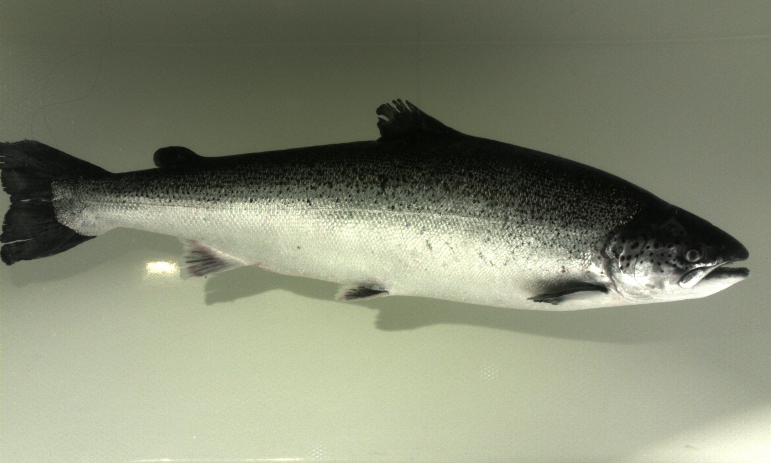
\includegraphics[width=.98\linewidth]{images/literature/original_fish}
        \caption{Original Image}
    \end{subfigure}%
    \begin{subfigure}{.5\textwidth}
        \centering
        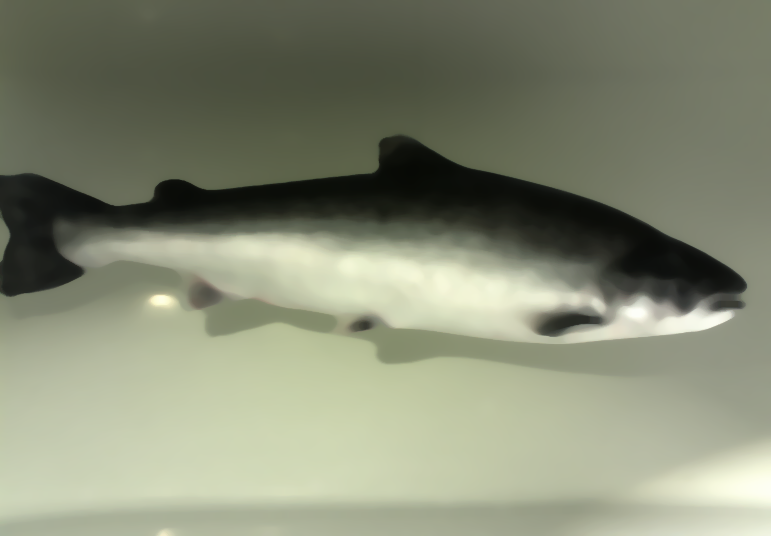
\includegraphics[width=.98\linewidth]{images/literature/medianblur}
        \caption{Median Filter}
    \end{subfigure}
    \caption{Example of median filtering}
    \label{fig:median_filter}
\end{figure}

It is seen from the images in figure \ref{fig:median_filter} that both the background and all patterns on the fish are smoothed out, while the edges are preserved. Small particles is also removed; for example it is possible to see that some of the white reflections under the fish is gone. The median filter used on this image has kernel size 11, and it was filtered 2 times in a row. When filtering several times in a row instead of increasing the kernel size the image will not get as blurry and small particles will still be removed.


\subsubsection{Bilateral Filter}
The bilateral filter is, just as the median filter, a nonlinear digital filter used to remove noise, while preserving sharp edges. Each pixel in an image is replaced by a weighted average of intensity values from neighboring pixels. The weight does not only depend on distance, but also on the radiometric differences such as color intensity or depth distance. 

\begin{figure}[h]
    \centering
    \begin{subfigure}{0.5\textwidth}
        \centering
        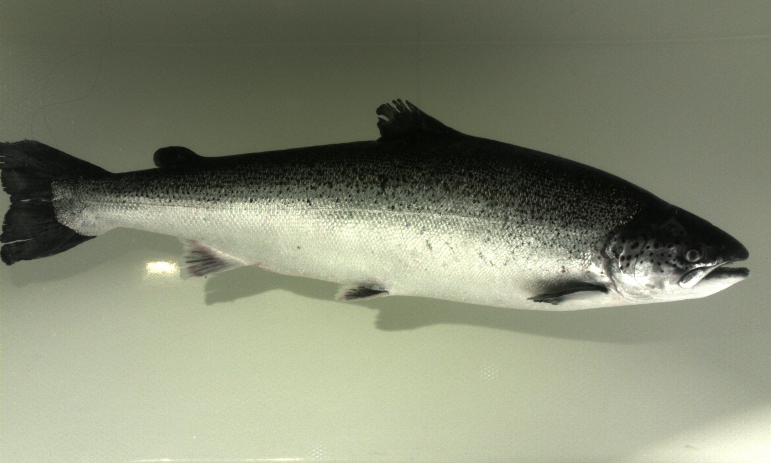
\includegraphics[width=.98\linewidth]{images/literature/original_fish}
        \caption{Original Image}
    \end{subfigure}%
    \begin{subfigure}{.5\textwidth}
        \centering
        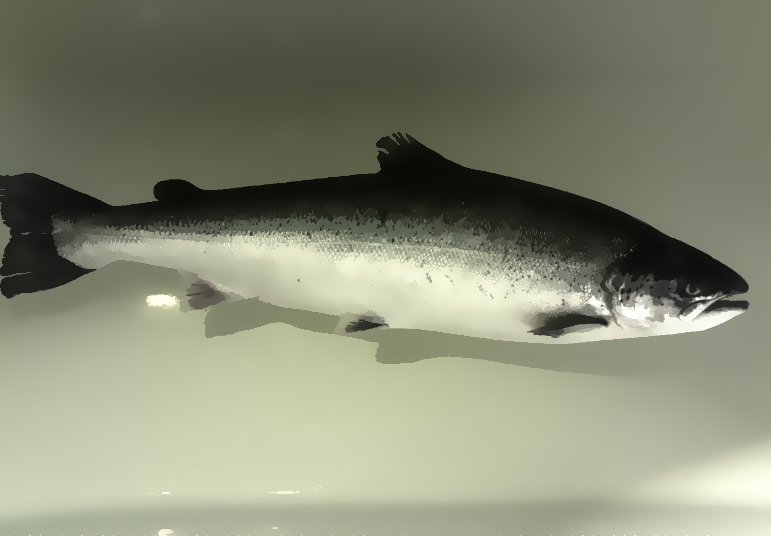
\includegraphics[width=.98\linewidth]{images/literature/bilateralblur}
        \caption{Bilateral Filter}
        \label{fig:bilateral_filter_b}
    \end{subfigure}
    \caption{Example of bilateral filtering}
    \label{fig:bilateral_filter}
\end{figure}

From figure \ref{fig:bilateral_filter} it is possible to see that the edges are well preserved and small imperfections are blurred out. This filter also increases the intensity in the image. Figure \ref{fig:bilateral_filter_b} was filtered with kernel size 11, and it was filtered 5 times in a row.


\subsection{Shadow Removal}
There are few open source algorithms for shadow removal. There are some advanced explanations for shadow removal, but they do not always work properly. Shadow removal can be useful when reconstructing an image or when detecting objects. 
Simple shadow removal can be done by transforming the color space of the image from RBG to HSV and then setting the value component of each pixel to a constant value. What this really does is even out all grey tones in the image, as is shown in figure \ref{fig:shadow_removal}.

\begin{figure}[h]
    \centering
    \begin{subfigure}{0.5\textwidth}
        \centering
        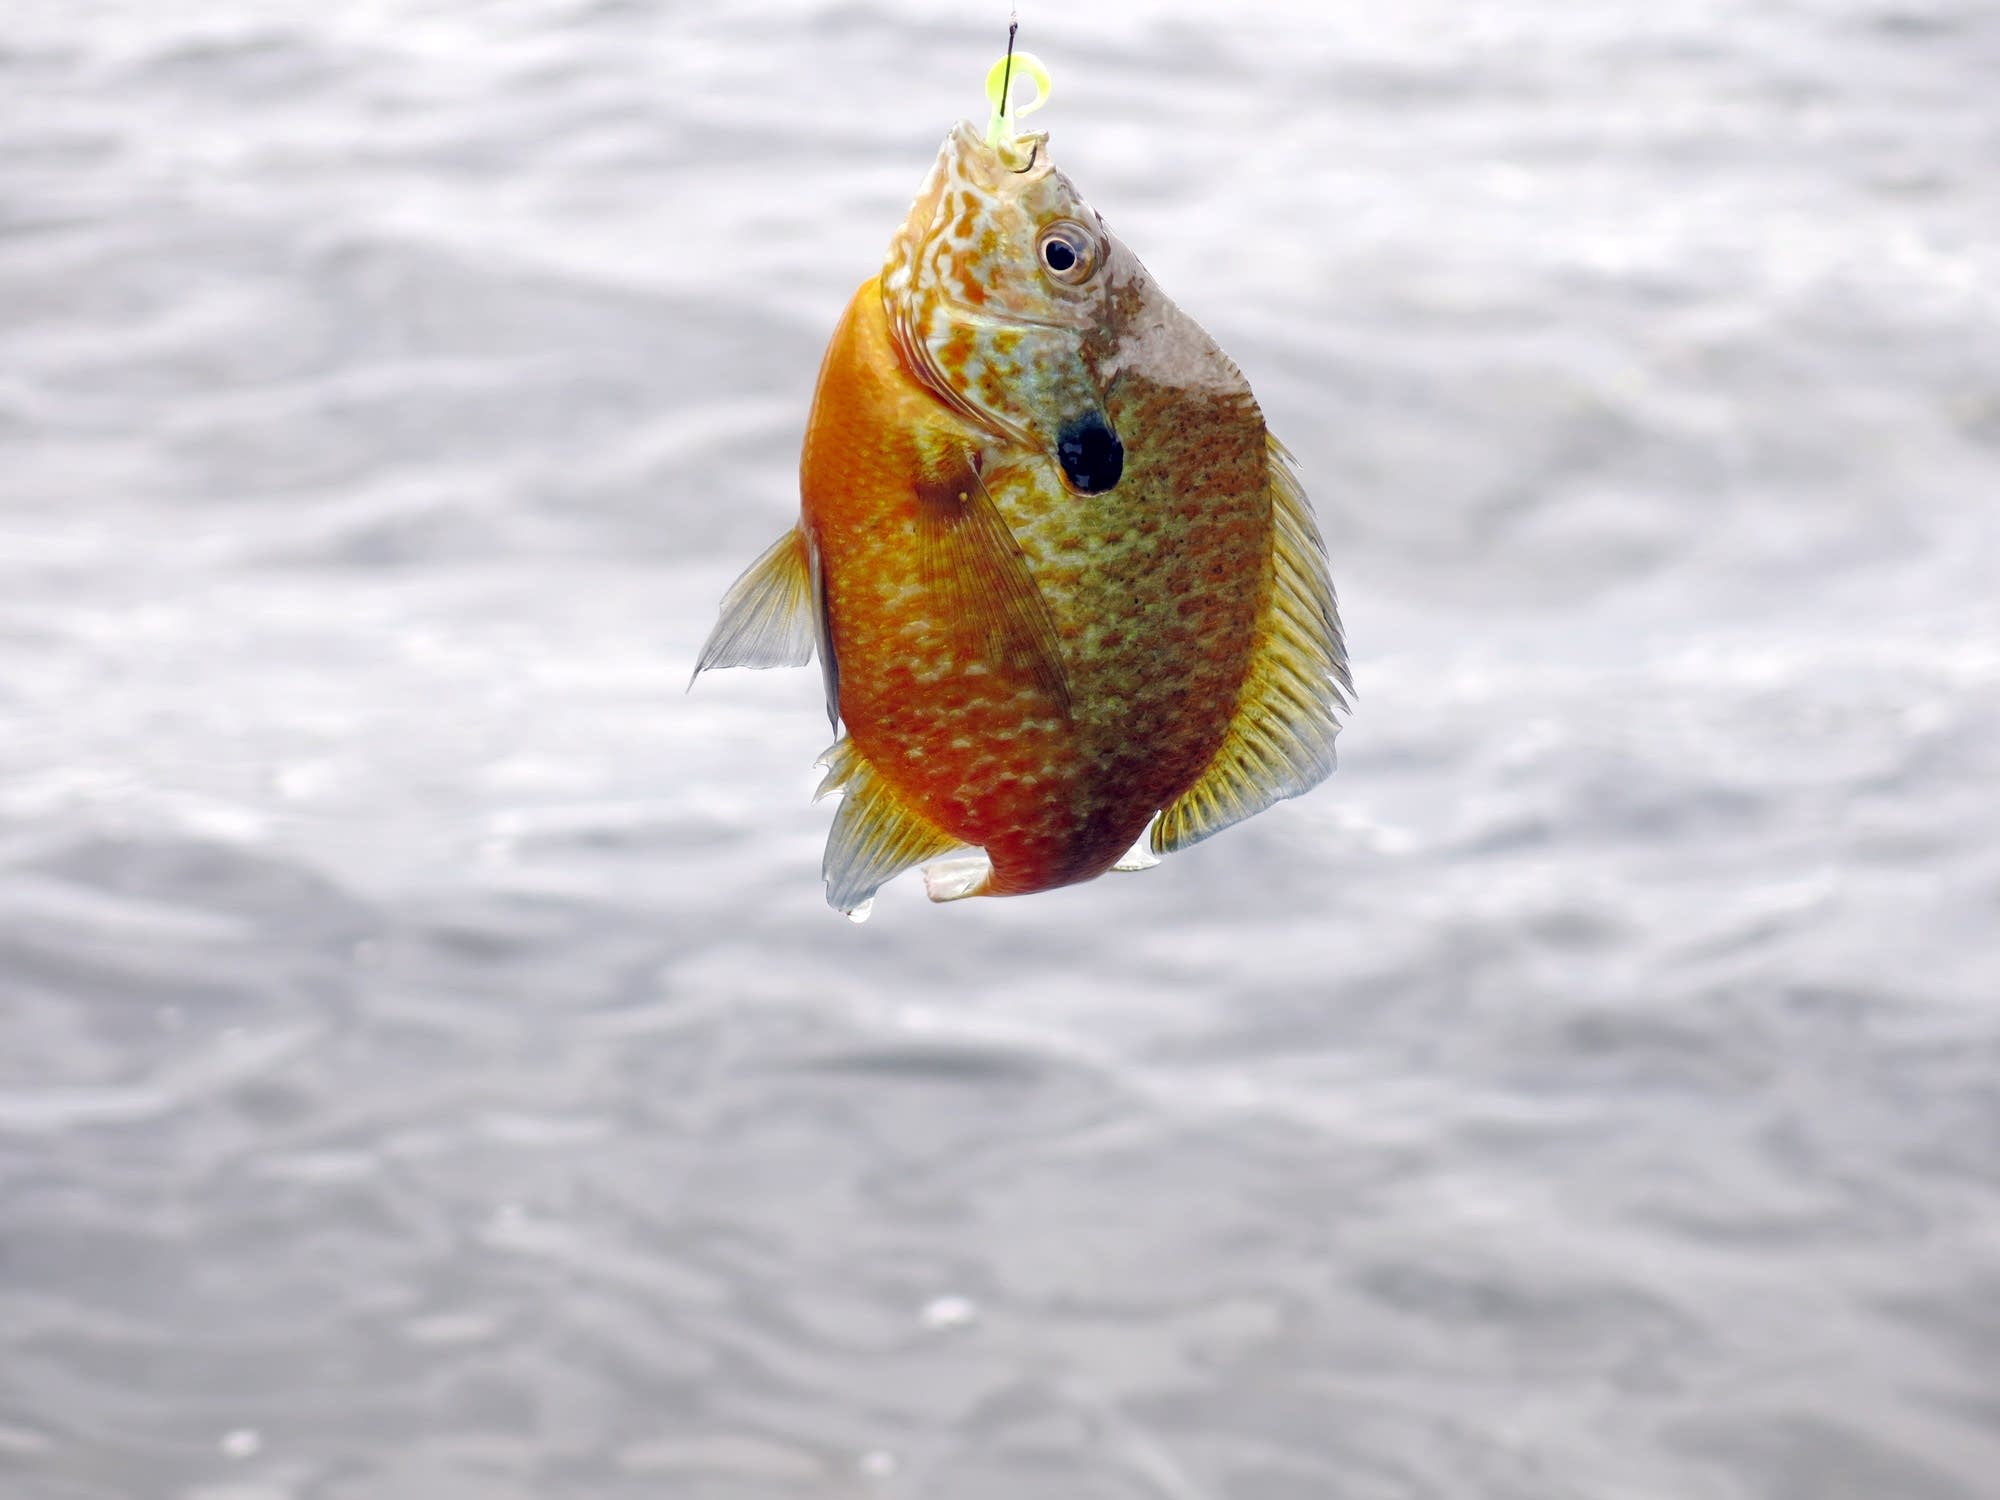
\includegraphics[width=.9\linewidth]{images/literature/colorfish}
        \caption{Original Image}
    \end{subfigure}%
    \begin{subfigure}{.5\textwidth}
        \centering
        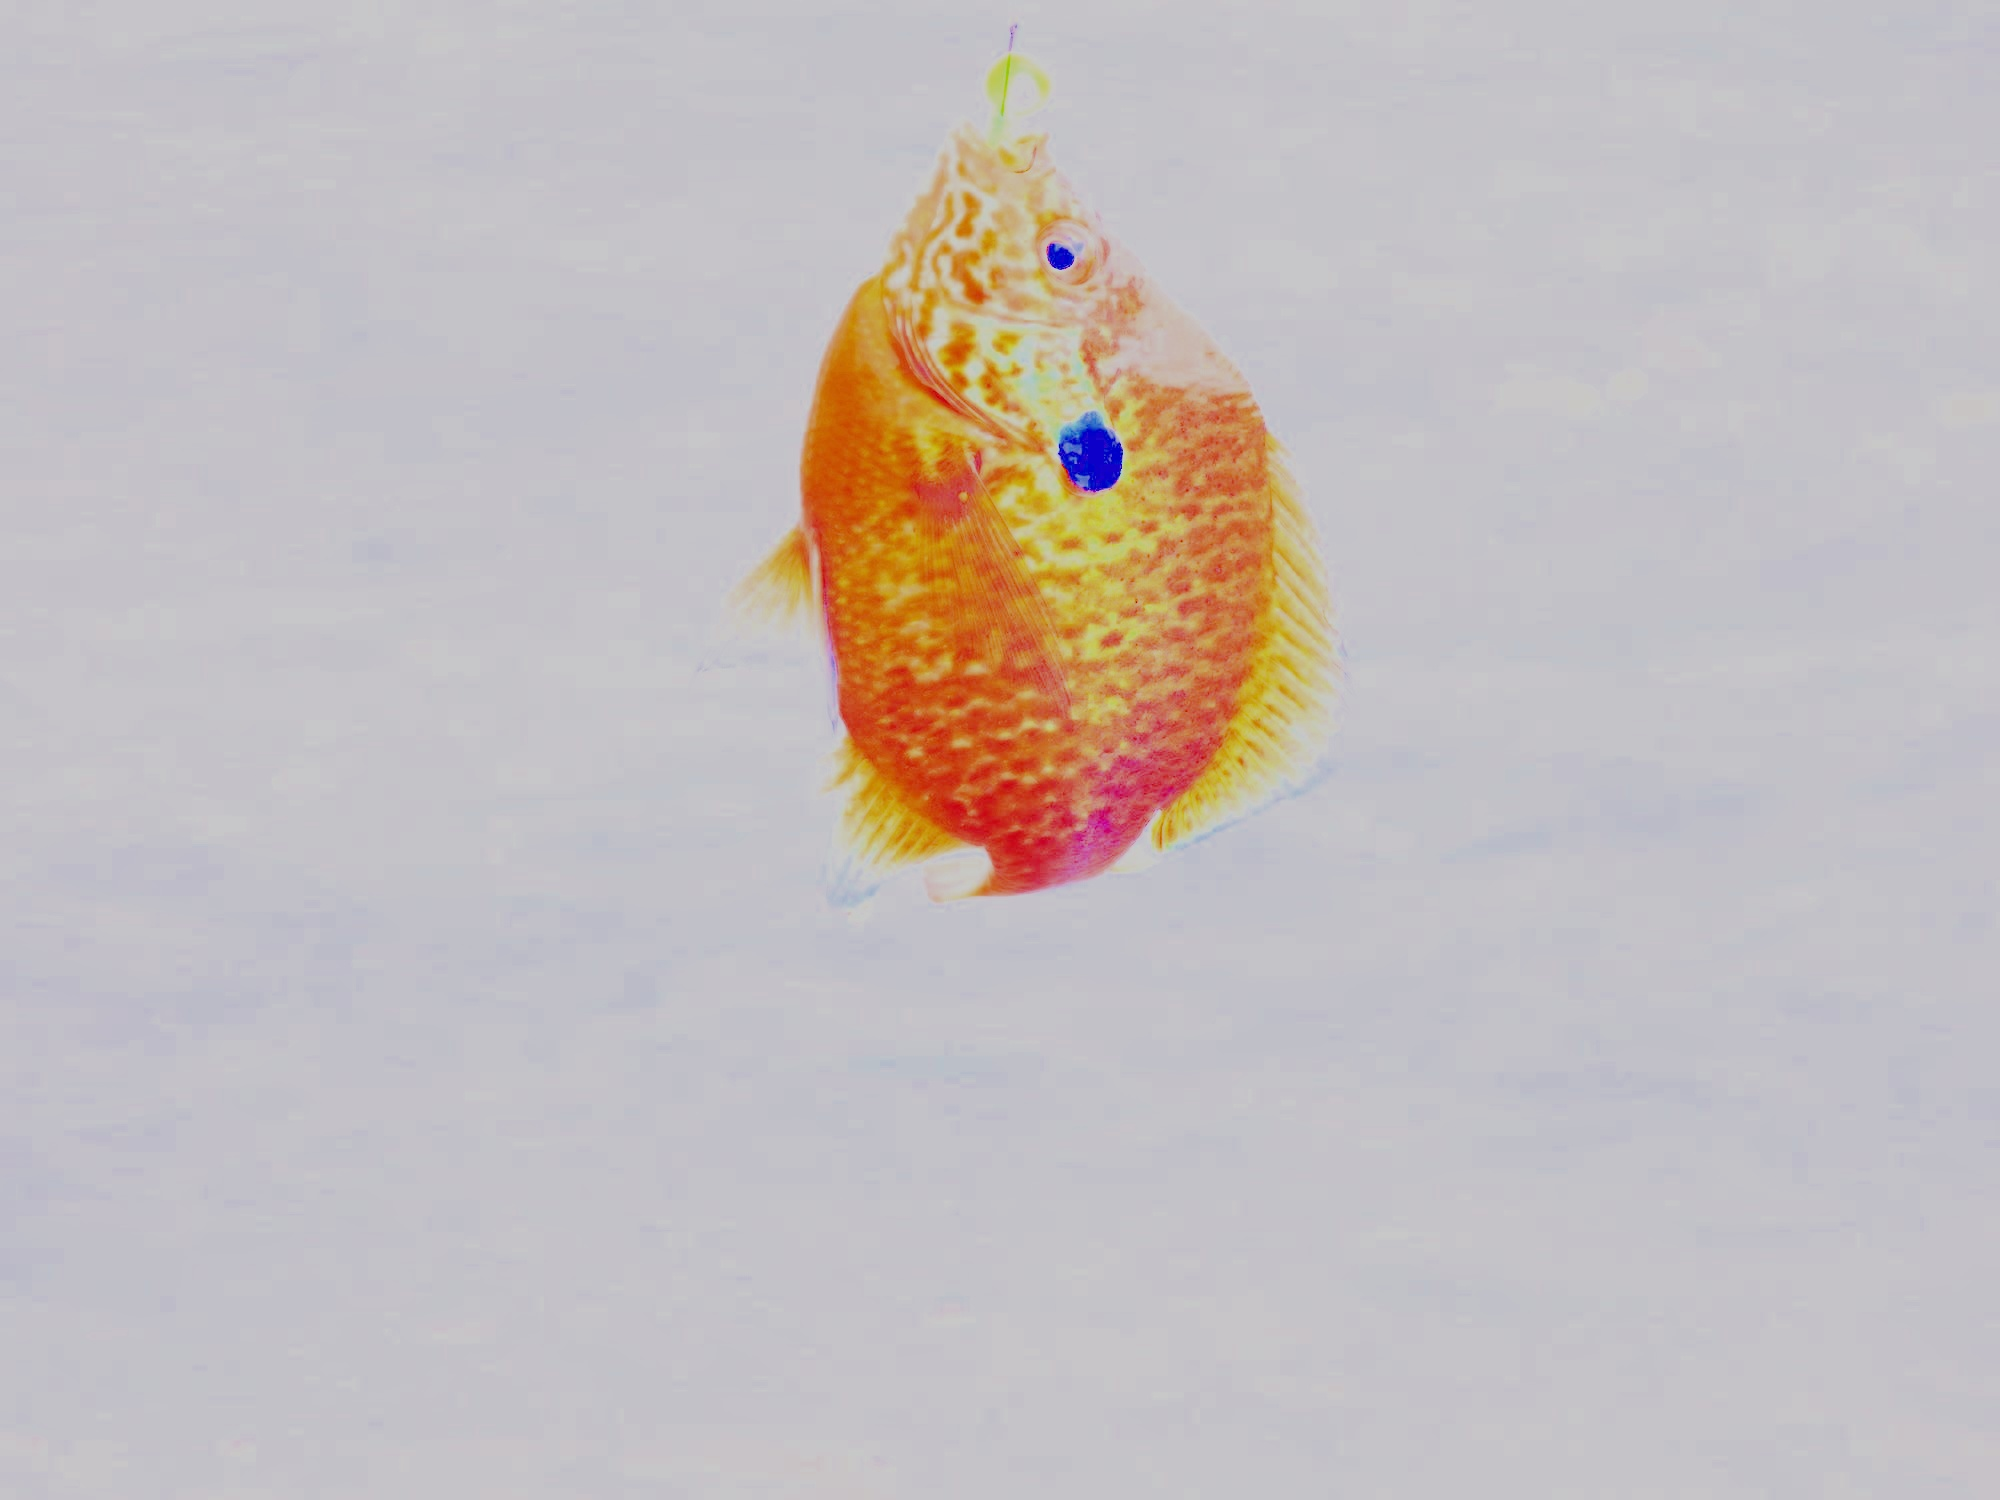
\includegraphics[width=.9\linewidth]{images/literature/shadow_removal}
        \caption{Shadow Removal}
    \end{subfigure}
    \caption{Example of shadow removal}
    \label{fig:shadow_removal}
\end{figure}

In figure \ref{fig:shadow_removal} it is shown that the colors of the fish is preserved, while all the shadows and blurry background in grey tones is evened out. In this example the value component is set to 200.

This type of simple shadow removal can be very useful, but for the image in figure \ref{fig:median_filter} the fish is not colorful enough for the technique to remove the shadows only.


%%%%%%%%%%%%%%%%%%%%%%%%%%%%%%%%%%%%%%%%%%%%%%%%%%%%%%%%%%%%%%%%%%%%%%


\subsection{Filtering in the Frequency Domain}

The frequency domain is a space in which the image value at some pixel represents the amount that the intensity values vary over some distance. Changes done in the frequency domain affects the rate at which the intensity values are changing in the spatial domain. 
The Fourier Transform is mostly used to convert images from the spatial domain into the frequency domain, and the Inverse Fourier Transform is used to convert the other way. 
Filtering in the frequency domain is mostly used for removing continuous patters that occur in the spatial domain image.
Filtering in the frequency domain is also faster than running an averaging filter in the spatial domain, especially as the kernel size increases. 

In the frequency domain the spectrum is used to see the amplitudes of the sinusoids. A large amplitude implies a pattern in the spatial image. By removing the wanted amplitudes from the spectrum and using the Inverse Fourier Transform, the pattern from the amplitudes will be removed.
By removing certain frequencies in the frequency domain it is possible to remove patters like stripes on old images or light scattering in underwater images.


\subsubsection{Light scattering}
There are many problems with underwater image processing due to the light propagation in the water medium. The physical properties of water cause degradation effects not present in images taken in air. The water absorbs light and therefore limits the visibility distance, and it also causes scattering, which changes the direction of the light path. This influences the overall performance of underwater imaging systems. Forward scattering is the spreading of light from an object towards the camera, while backward scattering is the light reflected by the water towards the camera before it actually reaches an object. Backward scattering reduces the contrast of the image, and is seen as sunbeams on the image. Scattering comes from not only the water, but all particles in the water. \cite{article:underwater_image_processing}

\begin{figure}[h]
    \centering
    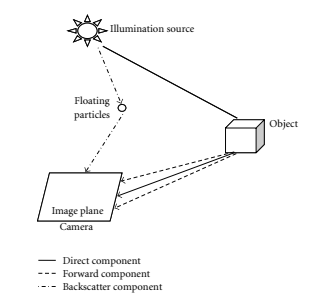
\includegraphics[width=0.7\textwidth]{images/image_from_paper}
    \caption{Explanation of scattering from (Raimondo Schettini and Silvia Corchs, 2010, p. 3)}
    \label{fig:image_from_paper}
\end{figure}

Filtering in the frequency domain could be a solution to reduce the scattering in underwater images.


%%%%%%%%%%%%%%%%%%%%%%%%%%%%%%%%%%%%%%%%%%%%%%%%%%%%%%%%%%%%%%%%%%%%%%


\subsection{Morphological Operators}

Morphology is a wide set of operations that process images based on shape. The operators apply a structuring element to an input image, and the value of each pixel in the output image is based on a comparison of the pixel with its neighbors. The structuring element is chosen by size and shape, and therefore determines what shapes the operation is sensitive towards. 
The shape of the structuring element can be chosen as flat or non-flat. Examples of flat structuring elements are ellipse, cross or rectangle, as shown below. Non-flat structuring elements have different weighting on the neighboring pixels. 

\noindent Ellipse: 
$\begin{bmatrix}
    0 & 0 & 1 & 0 & 0 \\
    1 & 1 & 1 & 1 & 1 \\
    1 & 1 & 1 & 1 & 1 \\
    1 & 1 & 1 & 1 & 1 \\
    0 & 0 & 1 & 0 & 0
\end{bmatrix}$ 
Cross: 
$\begin{bmatrix}
    0 & 0 & 1 & 0 & 0 \\
    0 & 0 & 1 & 0 & 0 \\
    1 & 1 & 1 & 1 & 1 \\
    0 & 0 & 1 & 0 & 0 \\
    0 & 0 & 1 & 0 & 0 
\end{bmatrix}$
Rect: 
$\begin{bmatrix}
    1 & 1 & 1 & 1 & 1 \\
    1 & 1 & 1 & 1 & 1 \\
    1 & 1 & 1 & 1 & 1 \\
    1 & 1 & 1 & 1 & 1 \\
    1 & 1 & 1 & 1 & 1
\end{bmatrix}$

Example of non-flat structuring element:
$\begin{bmatrix}
    0 & 0 & 1 & 0 & 0 \\
    0 & 1 & 2 & 1 & 0 \\
    1 & 2 & 4 & 2 & 1 \\
    0 & 1 & 2 & 1 & 0 \\
    0 & 0 & 1 & 0 & 0
\end{bmatrix}$ 

Morphological operators are useful for separating objects from each other, or merging objects together. It can also be used to remove small objects from an image, separate objects, merge objects, or to highlight certain objects.


\subsubsection{Dilate and Erode}
The most basic morphological operators are dilation and erosion. On gray-scale images dilation will add pixels on white object boundaries, while erosion will add pixels on black object boundaries.
\begin{itemize}
    \item Dilation: The value of the output pixel is the \textit{maximum} value of all pixels in the input pixels neighborhood. 
    \item Erosion: The value of the output pixel is the \textit{minimum} value of all pixels in the input pixels neighborhood. \cite{website:mathworks_dilation_erosion}
\end{itemize}

\begin{figure}[h]
    \centering
    \begin{subfigure}{0.33\textwidth}
        \centering
        
\includegraphics[width=.9\linewidth]{images/literature/star}
        \caption{Original Image}
    \end{subfigure}%
    \begin{subfigure}{.33\textwidth}
        \centering
        
\includegraphics[width=.9\linewidth]{images/literature/dilation}
        \caption{Dilation}
    \end{subfigure}%
    \begin{subfigure}{.33\textwidth}
        \centering
        
\includegraphics[width=.9\linewidth]{images/literature/erosion}
        \caption{Erosion}
    \end{subfigure}
    \caption{Example of dilation and erosion}
    \label{fig:star_dilate_erode}
\end{figure}



\subsubsection{Opening and Closing}
Opening and closing are combinations of dilation and erosion. Opening is the dilation of the erosion of an image, while closing is the erosion of the dilation of an image. 

\begin{figure}[h]
    \centering
    \begin{subfigure}{0.33\textwidth}
        \centering
        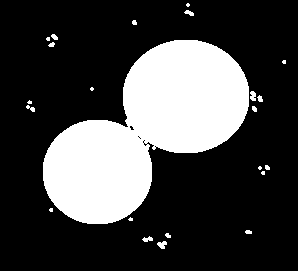
\includegraphics[width=.9\linewidth]{images/literature/dots}
        \caption{Original Image}
    \end{subfigure}%
    \begin{subfigure}{.33\textwidth}
        \centering
        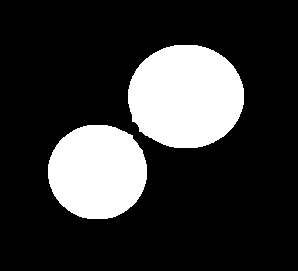
\includegraphics[width=.9\linewidth]{images/literature/opening}
        \caption{Opening}
    \end{subfigure}%
    \begin{subfigure}{.33\textwidth}
        \centering
        
\includegraphics[width=.9\linewidth]{images/literature/closing}
        \caption{Closing}
    \end{subfigure}
    \caption{Example of opening and closing}
    \label{fig:dots_opening_closing}
\end{figure}

Opening and closing assumes bright objects on a dark background. When opening an image, small objects will be removed and objects close to each other will be separated. When closing an image, objects close to each other will be closed together into one object. See figure \ref{fig:dots_opening_closing}.


%%%%%%%%%%%%%%%%%%%%%%%%%%%%%%%%%%%%%%%%%%%%%%%%%%%%%%%%%%%%%%%%%%%%%%


\newpage
\subsection{Thresholding}

Thresholding is a simple image segmentation method. It is mostly used on grayscale images to obtain a binary image. In its simples form it replaces each pixel with black if the the intensity is less than some fixed threshold value, and with white if the intensity is above the threshold value. 
The threshold value can be set manually, or chosen by the computer, depending on the threshold method used. 

Thresholding is most used to detect objects from the background.

\subsubsection{Adaptive Thresholding}
Sometimes the intensity of both the object and the background changes rapidly throughout the image. This makes it hard to set a threshold value that holds for the entire image. In these situations local thresholding is the solution. Local (adaptive) thresholding runs through each pixel and chooses a threshold value based on each pixel's neighborhood. How the threshold is chosen is up to the user to decide, but most common is the median value or the Gaussian mean value.

